%%%%%%%%%%%%%%%%%%%%%%%%%%%%%%%%%%%%%%%%%%%%%%%%%%%%%%%%%%%%%%%%%%%%%%%%%%%%%%%%%%%%%%%%%%%%%%%%%%%%%%%%%%%%%%%%%%%%%%%%%%%%%%%%%%%%%%%%%%%%%%%%%%%%%%%%%%%
% This is just an example/guide for you to refer to when submitting manuscripts to Frontiers, it is not mandatory to use Frontiers .cls files nor frontiers.tex  %
% This will only generate the Manuscript, the final article will be typeset by Frontiers after acceptance.   
%                                              %
%                                                                                                                                                         %
% When submitting your files, remember to upload this *tex file, the pdf generated with it, the *bib file (if bibliography is not within the *tex) and all the figures.
%%%%%%%%%%%%%%%%%%%%%%%%%%%%%%%%%%%%%%%%%%%%%%%%%%%%%%%%%%%%%%%%%%%%%%%%%%%%%%%%%%%%%%%%%%%%%%%%%%%%%%%%%%%%%%%%%%%%%%%%%%%%%%%%%%%%%%%%%%%%%%%%%%%%%%%%%%%

%%% Version 3.4 Generated 2022/06/14 %%%
%%% You will need to have the following packages installed: datetime, fmtcount, etoolbox, fcprefix, which are normally inlcuded in WinEdt. %%%
%%% In http://www.ctan.org/ you can find the packages and how to install them, if necessary. %%%
%%%  NB logo1.jpg is required in the path in order to correctly compile front page header %%%

\documentclass[utf8]{FrontiersinHarvard} % for articles in journals using the Harvard Referencing Style (Author-Date), for Frontiers Reference Styles by Journal: https://zendesk.frontiersin.org/hc/en-us/articles/360017860337-Frontiers-Reference-Styles-by-Journal
%\documentclass[utf8]{FrontiersinVancouver} % for articles in journals using the Vancouver Reference Style (Numbered), for Frontiers Reference Styles by Journal: https://zendesk.frontiersin.org/hc/en-us/articles/360017860337-Frontiers-Reference-Styles-by-Journal
%\documentclass[utf8]{frontiersinFPHY_FAMS} % Vancouver Reference Style (Numbered) for articles in the journals "Frontiers in Physics" and "Frontiers in Applied Mathematics and Statistics" 

%\setcitestyle{square} % for articles in the journals "Frontiers in Physics" and "Frontiers in Applied Mathematics and Statistics" 
\usepackage{url,hyperref,lineno,microtype,subcaption}
\usepackage[onehalfspacing]{setspace}
%\usepackage{tabulary}
\usepackage{tabularx}
\linenumbers


% Leave a blank line between paragraphs instead of using \\


\def\keyFont{\fontsize{8}{11}\helveticabold }
\def\firstAuthorLast{Yamba {et~al.}} %use et al only if is more than 1 author
\def\Authors{Edmund I. Yamba\,$^{1,*}$, Kingsley Badu\,$^{2}$, Peter Haddawy\,$^{3}$, Thomas A. Kyeimiah\,$^{4}$, Nathaniel O. Abrokwah\,$^{5}$, Stephen Asare\,$^{1}$, Franklin Asiedu-Bekoe\,$^{6}$ and Leonard K. Amekudzi\,$^{1}$}
% Affiliations should be keyed to the author's name with superscript numbers and be listed as follows: Laboratory, Institute, Department, Organization, City, State abbreviation (USA, Canada, Australia), and Country (without detailed address information such as city zip codes or street names).
% If one of the authors has a change of address, list the new address below the correspondence details using a superscript symbol and use the same symbol to indicate the author in the author list.
\def\Address{$^{1}$Department of Meteorology and Climate Science, Kwame Nkrumah University of Science and Technology (KNUST), Kumasi, Ghana. \\
$^{2}$ Department of Theoretical and Applied Biology, Kwame Nkrumah University of Science and Technology (KNUST), Kumasi, Ghana.\\
$^{3}$ Faculty of informatics, University of Bremen, Bremen Germany\\
$^{4}$ Department of Atmospheric and Oceanic Sciences, McGill University, Canada.\\
$^{5}$ Department of Atmospheric Sciences, University of Wyoming, USA.\\
$^{6}$ Public Health Directorate, Ghana Health Service, Accra, Ghana.}
% The Corresponding Author should be marked with an asterisk
% Provide the exact contact address (this time including street name and city zip code) and email of the corresponding author
\def\corrAuthor{Department of Meteorology and Climate Science, PMB, University Post Office, KNUST, Kumasi}

\def\corrEmail{eiyamba@knust.edu.gh}

\begin{document}
\onecolumn
\firstpage{1}

%\title[Climate-based Malaria Modeling]{Climate-based modelling of the thrivability and expansion ranges of malaria vectors for enhanced surveillance and control} 

\title[Climate-based Malaria Modeling]{Modeling Climate-Induced Changes in Vectorial Capacity of Malaria Vectors for Enhanced Vector Surveillance and Control} 

\author[\firstAuthorLast ]{\Authors} %This field will be automatically populated
\address{} %This field will be automatically populated
\correspondance{} %This field will be automatically populated

\extraAuth{}% If there are more than 1 corresponding author, comment this line and uncomment the next one.
%\extraAuth{corresponding Author2 \\ Laboratory X2, Institute X2, Department X2, Organization X2, Street X2, City X2 , State XX2 (only USA, Canada and Australia), Zip Code2, X2 Country X2, email2@uni2.edu}


\maketitle


\begin{abstract}
Malaria remains a significant threat to Sub-Saharan Africa, where approximately 94\% of malaria cases and deaths occur. Ghana, however, has made strides in reducing malaria prevalence and fatalities through its National Malaria Elimination Programme (NMEP), which sets ambitious targets: achieving a 100\% reduction in mortality by 2028 and halving cases compared to 2022 figures. Crucial to attaining these goals is a data-driven approach, particularly in strengthening malaria surveillance. Unfortunately, Ghana's current surveillance system is inadequate, mainly reliant on healthcare facility-based reporting, which has limitations such as underrepresentation of rural areas and the knowledge gaps among healthcare providers. Furthermore, climate variables significantly impact malaria transmission, yet existing surveillance systems in Ghana do not fully integrate climate data. To address these gaps, a study proposes using climate suitability data to predict the survival rates, distribution, and transmission capacity of malaria vectors across Ghana. By identifying regions where Anopheles mosquitoes can thrive and expand, policymakers, including the NMEP, can tailor targeted vector surveillance and control strategies. This approach holds the potential to enhance malaria control, reducing its public health burden in Ghana. 
\tiny
 \keyFont{ \section{Keywords:} Climate-based, Modeling, malaria, vector, surveillance, decision-making, Ghana} %All article types: you may provide up to 8 keywords; at least 5 are mandatory.
\end{abstract}

\section{Introduction}

Despite efforts to eradicate malaria in sub-Saharan Africa, the African continent still accounts for over 94\% of all cases and fatalities worldwide, and no progress has been made since 2017 toward eradication (WHO 2022). The high burden is largely explained by the region's favorable climate for effective malaria parasites and their vectors to thrive and dominate (Sinka et al. 2010). Anthropogenic climate change adds to the burden, by changing the suitability of landscapes for the proliferation of Anopheles mosquitoes (Afrane et al., 2012; Colón-González et al., 2021). 


Unfortunately, the current malaria surveillance system in the region is very weak, mainly reliant on healthcare facility-based reporting, which has significant limitations such as underrepresentation of rural areas where healthcare is totally absent or very weak. The surveillance data are typically collected in pieces by different stakeholders and aggregated across the country. Such data are challenging to use to keep track of the disease trends, identify the most afflicted areas or population groups and develop efficient and accessible interventions. Again, malaria transmission is mainly driven by the weather and climate of an area, yet the disease surveillance systems do not operationally use weather and climate impact information to inform intervention. Hence, the absence of a full-scale and robust malaria surveillance and forecasting system is the missing piece of the puzzle that prevents the transition from ad hoc malaria control to elimination in the region. Taking advantage of malaria transmission being climate sensitive and following best practices in weather forecasting, this project seeks to provide real-time malaria surveillance and forecasting information using a more intelligent data-driven surveillance mechanism that is faster, safer, and cheaper. Our idea involves the use of dynamical malaria modeling, incorporating biological, environmental and climatic data, to produce malaria information that can be forecasted, geolocated and mapped in real-time. Our aim is to assist Ghana’s National Malaria Elimination Programme (NMEP) achieve its ambitious target of reducing malaria mortality by 100\% and cases by 50\% by 2028 using the 2022 figures as the baseline. Hence, the model will be operationally run on good computer systems at the Kwame Nkrumah University of Science and Technology (KNUST), Ghana providing forecast information such as malaria case counts, vectorial capacity, extrinsic incubation period,  and infectious mosquito bites across Ghana on a spatial scale of 5km and on subseasonal to seasonal time scale. With this real-time surveillance information, the NMCP and other stakeholders involved in malaria decision-making can target malaria control resources such as insecticide treated bed nets, diagnostics and medicines to areas where they are needed most as well as evaluate the impact of malaria control programmes to know which and where it works best. Ultimately, our work will support cost-effective malaria intervention, significantly lower malaria morbidity and mortality and influence better policy making for malaria control in Ghana. Our work will also support the World Health Organization global strategy for malaria control and elimination and contribute to achieving the Sustainable Development Goals (SDGs) such as good health and well-being (SDG3), poverty eradication (SDG1), and reduced inequality (SDG10). 

\noindent Malaria is an infectious disease, transmitted to humans through the bites of infected female Anopheles mosquitoes \citep{world2022world}. Malaria is life-threatening with a high global burden in sub-Saharan Africa \citep{world2022world}. According to \cite{world2022world}, about 95\% of the global malaria cases and deaths in 2020 occurred in this region, with children under five years of age accounting for 80\% of the deaths. Women (especially pregnant women), children and the poorest communities are the most vulnerable to malaria. For instance, malaria affects children's mental and physical development, keeps older children out of school, adults out of work, contributing to the cycle of poverty and negatively impacting the prosperity of individuals and communities. Significant portions of hospital admissions are due to malaria, stressing the already fragile health system. With a stagnation in control since 2017, malaria remains a threat to millions of Ghanaians and sub-Saharan Africans on the whole \citep{world2022world}.

In sub-Saharan Africa, the impact of climate on malaria vectors and disease transmission has been widely acknowledged. Temperature, rainfall, humidity, land cover change, and vector ecology are key drivers of malaria in both endemic and epidemic areas \citep{yamba2023climate,yamba2020monthly}. Rainfall, for instance, provides the environment for vector breeding and relative humidity of at least 60\% appears necessary for vector survival \citep{ermert2011development, tompkins2013regional}. Rainfall and relative humidity, therefore, affects the availability, persistence and dimensions of Anopheles vectors and their larval habitats \citep{tompkins2013regional,asare2016breeding}. Temperature, on the other hand, drives the physiological processes of mosquitoes and in the face of temperature change, mosquitoes make necessary physiological adjustments to live either by evolving and adapting to the changes or move to a more suitable area permanently or temporarily \citep{buckley2016extreme,villena2022temperature,ryan2023mapping}. For instance, the physiological processes of mosquitoes highly fluctuates or constrained by ambient temperature and the rates of the biological and biochemical processes shift with temperature, impacting traits that impact fitness such as development and survival rates \citep{villena2022temperature,abram2017behavioural}. Thus temperature contributes to the observed dynamics and distributions of populations of mosquitoes. Anthropogenic climate change adds to the challenge of eliminating malaria by changing the suitability of landscapes for the proliferation of the Anopheles mosquitoes \citep{colon2021projecting}. As climate change alters temperatures and weather patterns across the region, the geographic areas where malaria parasites and  mosquitoes thrive also changes altering the timings and length of malaria transmission seasons. 



The WHO Global Technical Strategy (GTS) for malaria sets a goal to reduce case incidence and malaria deaths by 90\% by the year 2030 referencing 2015 levels. These targets have been missed by 37\% and 22\% respectively (WHO, 2020) because malaria-determining factors such as climate information, land use/cover change, resistance (parasite, insecticide, drug), accurate diagnosis, and other related environmental factors are not operationally used in African health decision-making processes.


Thus, there is an information gap on the potential impact of climate on malaria vectors thrivability and expansion ranges in Ghana as well as how climate change induces changes in malaria transmission in the country. This gap in information to action cycle is a significant challenge that hinders effective decision-making as far as vector control is concerned.
\noindent To improve malaria surveillance and support cost-effective malaria intervention strategies we provide the current and future thrivability and expansion range of malaria vectors over Ghana based on climate suitability. Specifically, we used potential climate impact information to predict current and future survival rates, distribution densities and  transmission capacity of malaria vectors across Ghana. Using these indices, we ranked spatio-temporally geographic regions where climates proxies provide suitable conditions for the Anopheles mosquitoes to thrive and expand. This gives us a clear picture of who is suffering most from the disease and where trends are occurring. With this information, the NMEP and allied policy makers can design targeted vector surveillance and control strategies to eliminate malaria in Ghana. This study holds the potential to significantly enhance malaria control strategies, ultimately reducing the burden of the disease on public health and society at large. \\

\section{Data and Methods}
\subsection{Study area}

\begin{figure}[ht]
\begin{center}
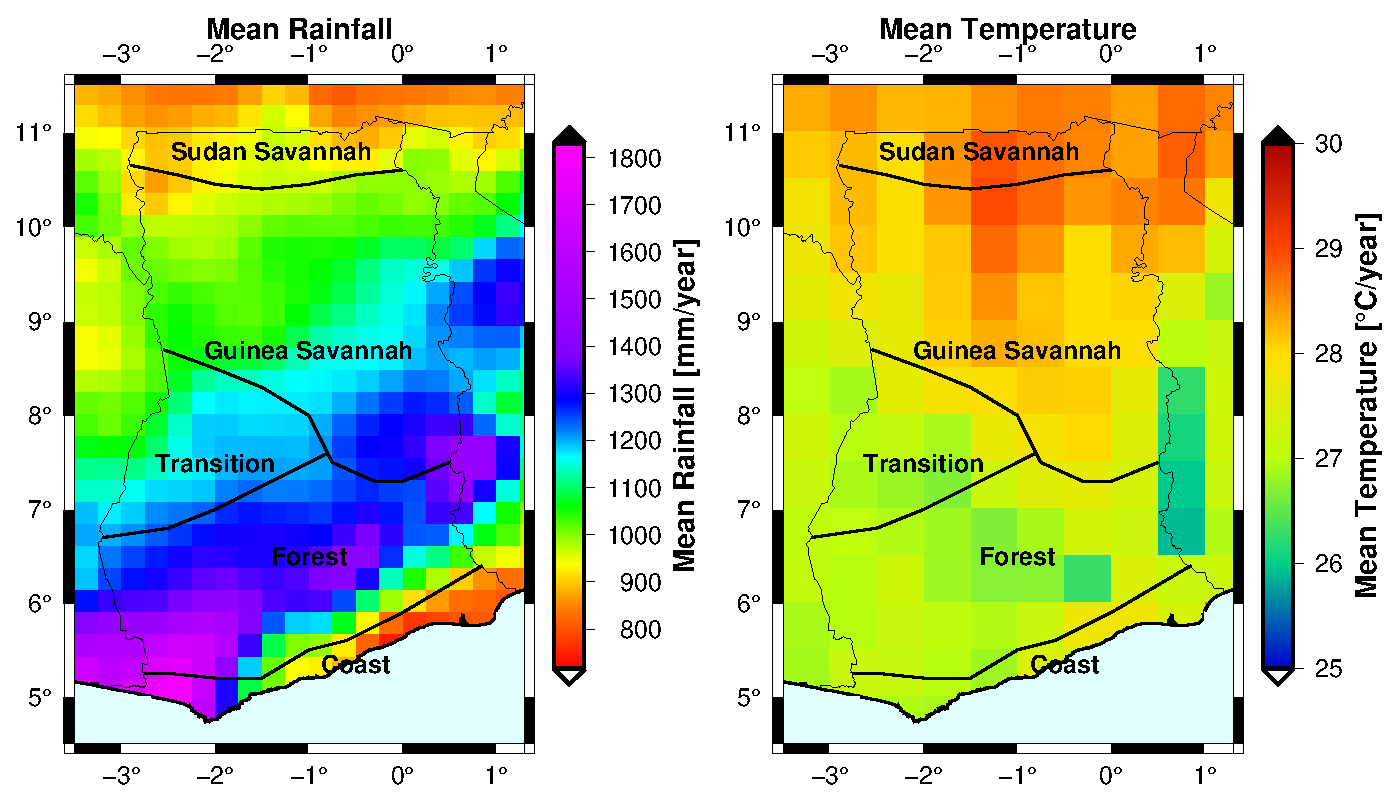
\includegraphics[width=15cm,height=9cm]{RRTmclimmap.eps}
\caption{The map of Ghana showing the ago-climatic zones as well as spatial distribution of annual total rainfall and temperature. Source: \citep{yamba2023revisiting}}
\label{fig:3.0}
\end{center}
\end{figure}

Ghana is a West African country situated between latitudes 4.5\textsuperscript{o}N and 11.5\textsuperscript{o}N and longitude 3.5\textsuperscript{o}W and 1.5\textsuperscript{o}E (see Fig~\ref{fig:3.0}). The country has a tropical monsoon climate governed by the West African Monsoon (WAM) \citep{ansah2020meteorological,aryee2018development}. The monsoon climate is further categorized into five distinct agro-climatic zones namely Sudan Savannah, Guinea Savannah, Transition, Forest and Coastal zones \citep{yamba2023revisiting}. Each zone has a distinct climate features from others and hence influence malaria transmission differently \citep{yamba2023climate}. The northern Ghana, that encompasses the Sudan and Guinea savannah, is characterized by uni-modal rainfall distribution which starts from April through mid-October with peak rainfall in August or September \citep{yamba2023revisiting}. The southern Ghana, encompasing the Transition, forest, and coastal zones has a bi-modal rainfall distribution. The first season runs from March to July, with peak in June, while the second season runs from September to mid-November, with peak in October \citep{yamba2023revisiting}. Between December and February, the harmattan, a north-easterly desert wind, dominates the country. The harmattan winds are more prevalent in the north, lowering humidity and resulting in hotter days and cooler nights in this area of the country \citep{aryee2018development}.
% Add a writeup on the main vectors of malaria transmission in Ghana

\subsection{Data}
\textbf{Rainfall}\\
\noindent Daily rainfall data spanning the period 1991 -- 2020 was extracted from the Climate Hazards Group Infra-Red Precipitation (CHIRPs) \citep{funk2015climate} and used in this study. CHIRPS is a gridded satellite-gauge product with a high spatial resolution of 0.25\textsuperscript{o} by 0.25\textsuperscript{o} and available globally on a daily time scale from 1981 to the present. CHIRPS was chosen because it is built from a combination of satellite and quality-controlled in situ data from ground-based weather stations. Moreover, previous studies \citep{gleixner2020did,parsons2022evaluation,verdin2020development} have validated the products and found it to have very good correlation with ground-based observations and lower biases across Africa. \\

%\subsubsection{Temperature}
\textbf{Temperature}\\
Similarly, daily 2m temperature data covering the years 1991-2020 were obtained from the European Centre for Medium-Range Weather Forecasts (ECMWF) Re-Analysis, 5th generation (ERA5) \citep{hersbach2020era5} for this study. ERA5 is a gridded re-analysis product with a high spatial resolution of 0.25\textsuperscript{o} by 0.25\textsuperscript{o} and available globally on an hourly time scale from 1979 to the present. ERA5 was preferred to other temperature products because of its high temporal availability (hourly from 1979 to present) and high spatial resolution ( 0.25\textsuperscript{o} by 0.25\textsuperscript{o}). Besides, validation studies \citep{gleixner2020did, parsons2022evaluation} have widely recommended it for meteorological research across Africa. \\

\textbf{Predicted rainfall and temperature }\\
For future analysis, daily rainfall and temperature data spanning the period 2031 -- 2090 was extracted from the Coordinated Regional Climate Downscaling Experiment (CORDEX) simulation framework database. The CORDEX experiments consist of a different combinations of Global Climate Models (GCMs) and Reginal Climate Model (RCM) simulations for different future climate scenarios (forcings) namely RCP2.6 RCP4.5 and RCP8.5 as well as different ensemble members of the same GCM-RCM combinations. Rainfall and temperature output from Regional Model version 2015 (REMO2015) driven by MPI-ESM-LR was extracted and used in this work. The rainfall data is available for the Africa Domain at horizontal grid spacing of 0.22$^{\circ}$ by 0.22$^{\circ}$ spanning the period 1950 to 2100. We temporally validated different cordex model data against observations over Ghana and found good performance from the MPI-ESM-LR. Again, previous validation studies \citep{ilori2021evaluating} have found a good performance of the models in replicating rainfall and temperature over Africa.   

\subsection{Analysis}
We analyzed the impact of climate on the capacity of anopheles mosquitoes to thrive and transmit malaria using the Vectorial Capacity (VC) index.  VC is defined as the rate at which mosquitoes can transmit parasites to humans \citep{Shapiro2017}. VC depends on a number of entomological factors involved in malaria transmission cycle namely vector density in relation to man (m), survival rate of malaria vectors (P), man-biting frequency (a), length of the sporogonic cycle expressed as Extrinsic Incubation Period (EIP), proportion of anopheline vectors with sporozoites that are actually infective (b) and human-to-mosquito transmission efficiency (c). The combined effect of these factors is expressed mathematically  \citep{paaijmans2012warmer} as:  
\begin{equation}\label{vc}
	VC  = {\dfrac{ma^{2}bcP^{EIP}}{-In(P)}}
\end{equation}

\noindent  The survival rate of malaria vectors, P, is a function of temperature and expressed mathematically using Martens II temperature scheme \citep{ermert2011development,lunde2013malaria} as follows:
%\begin{equation}\label{p}
%p_i = -0.00082T_i^2 + 0.0367T_i + 0.522
%\end{equation}

\begin{equation}\label{p}
	p_i = exp(\frac{-1}{-4.4+1.31T_i-0.03T_i^2})
\end{equation}

\noindent where T\textsubscript{i} represents the air temperature the mosquitoes experience on daily basis. Similarly, the Extrinsic Incubation Period (EIP) is also a function of temperature and was calculated using the formulation proposed by \citep{detinova1962age}:
\begin{equation}\label{eip}
	EIP = {\dfrac{D_s}{T_i-T_s}}
\end{equation}
\noindent where $D_{s}$ represent the sporogonic cycle length in degree days, $T_{s}$ is the sporogonic temperature threshold and $T_{i}$ is the temperature experienced by mosquitoes on daily basis. The vector biting frequency (a) was adapted from \cite{ceccato2012vectorial} and calculated using the equation:
%\begin{equation}
%a_i = HBI\frac{(T_i - T_g)}{D_g} 
%\label{equ:a_i}
%\end{equation}

\begin{equation}
a_i = \frac{HBI}{(1+\frac{D_g}{T_i-T_g})}
\label{brate}
\end{equation}
where HBI is the human Blood Index, $T_g$ is the minimum temperature for the gonotrophic cycle and $D_g$ is the gonotrophic cycle length in degree days. \\

Temperature drives the physiological processes of mosquitoes and in the face of temperature change, mosquitoes make necessary physiological adjustments to live either by evolving and adapting to the changes or move to a more suitable area permanently or temporarily \citep{buckley2016extreme,villena2022temperature,ryan2023mapping}. Thus, the rate of the biological and biochemical processes of mosquitoes shift with temperature, impacting on mosquito traits such as development, biting rates (a), EIP and survival rates \citep{villena2022temperature,abram2017behavioural} as expressed in eqns \ref{brate}, \ref{eip} and \ref{p}.

Rainfall (RR) on the other hand, provides the environment for vector breeding and relative humidity of at least 60\% appears necessary for vector survival \citep{ermert2011development, tompkins2013regional}. Rainfall therefore, affects the availability, persistence and dimensions of Anopheles vectors and their larval habitats \citep{tompkins2013regional,asare2016breeding}. This impact is expressed as having a direct link with the vector density in relation to man (m) with Eqn~\ref{vc} being re-expressed as: 

\begin{equation}\label{vc2}
	VC  = {\dfrac{(RR*m)a^{2}bcP^{EIP}}{-In(P)}}
\end{equation}
\noindent where RR is the daily rainfall.\\

Details of the parameter constants and the literature references from which they were obtained are shown in Table~\ref{modelparameters}. 
\begin{table}[!ht]
\caption{Default values of the climate-independent malaria model parameters.}
\label{modelparameters}
\centering
\resizebox{\textwidth}{!}{
\begin{tabular}{|lccl|} 
 \hline
 \textbf{Parameter} & \textbf{Symbol} & \textbf{Value} & \textbf{Reference}\\ \hline
 Human Blood Index & $HBI$ & 0.8 & \citep{ermert2011development}\\  
 Minimum temperature for gonotrophic cycle & $T_g$ & 7.7 $^{\circ}$C & \citep{detinova1962age,ermert2011development,tompkins2013regional}\\  
 Gonotrophic cycle length in degree days & $D_g$ & 37.1 & \citep{detinova1962age,ermert2011development,tompkins2013regional}\\  
 Minimum temperature for sporogonic cycle & $T_s$ & 16 $^{\circ}$C & \citep{ermert2011development,tompkins2013regional}\\  
 Sporogonic cycle length in degree days & $D_s$ & 111.0 & \citep{detinova1962age,ermert2011development,tompkins2013regional}\\ 
Mosquito-to-human transmission efficiency & \textbf{b}    & $0.3$ & \citep{ermert2011development,tompkins2013regional}\\
Human-to-mosquito transmission efficiency  & \textbf{c}  &    $0.2$ & \citep{ermert2011development,tompkins2013regional}\\ 
Vector: Human ratio & \textbf{m}     & $4$ & \citep{ermert2011development,tompkins2013regional}\\ 
Probability that a vector feeds on a human host & \textbf{a} & see Eqn \ref{brate} & \citep{ceccato2012vectorial} \\
 \hline 
\end{tabular}}
\end{table}

The VC was then calculated using Eqn~\ref{{vc2}} with inputs from eqns \ref{p}, \ref{eip}, \ref{brate} and information in Table~\ref{modelparameters}. Using the outcome, we mapped out areas of suitable climate conditions for anopheles vectors to thrive and transmit malaria for enhance vector surveillance and control across Ghana. 
%%%%%%%%%%%%%%%%%%%%%%%%%%%%%%%%%%%%%%%%%%


\section{Results}
Figure \ref{fig:3:1} illustrates the monthly survival rates of malaria vectors, offering valuable insights into their regional variations. It can be seen that, the northern regions of the country exhibit the lowest survival rates during the months of February, March, April, and May, ranging from 0.6 to 0.8. Among these months, May stands out with a relatively higher survival rate, while March records the lowest survival rate in this period. Moving towards the southern regions, we observe a noticeable increase in survival rates, ranging from 0.78 to 0.8, with peaks observed in the extreme southwest. The months of November, December, and January follow a similar spatial pattern, but with an overall higher rate of survival compared to February, March, and April. During this period, survival rates range from 0.78 to 0.84, with the highest rates concentrated in the southwestern part of the country, reaching a peak of 0.84. June and October had similar characteristics, a relatively higher rates of vector survival than the mentioned months with rates ranging from 0.86 in the northern regions to 0.9 in the southern regions. Remarkably, the survival rates in July, August, and September are consistently the highest nationwide, peaking at an impressive 0.94. This finding underscores the significance of these months in terms of malaria vector survival and highlights the need for targeted interventions during this period. These findings provide valuable insights into the geographic and temporal variations in malaria vector survival rates.
\begin{figure}[ht]
\begin{center}
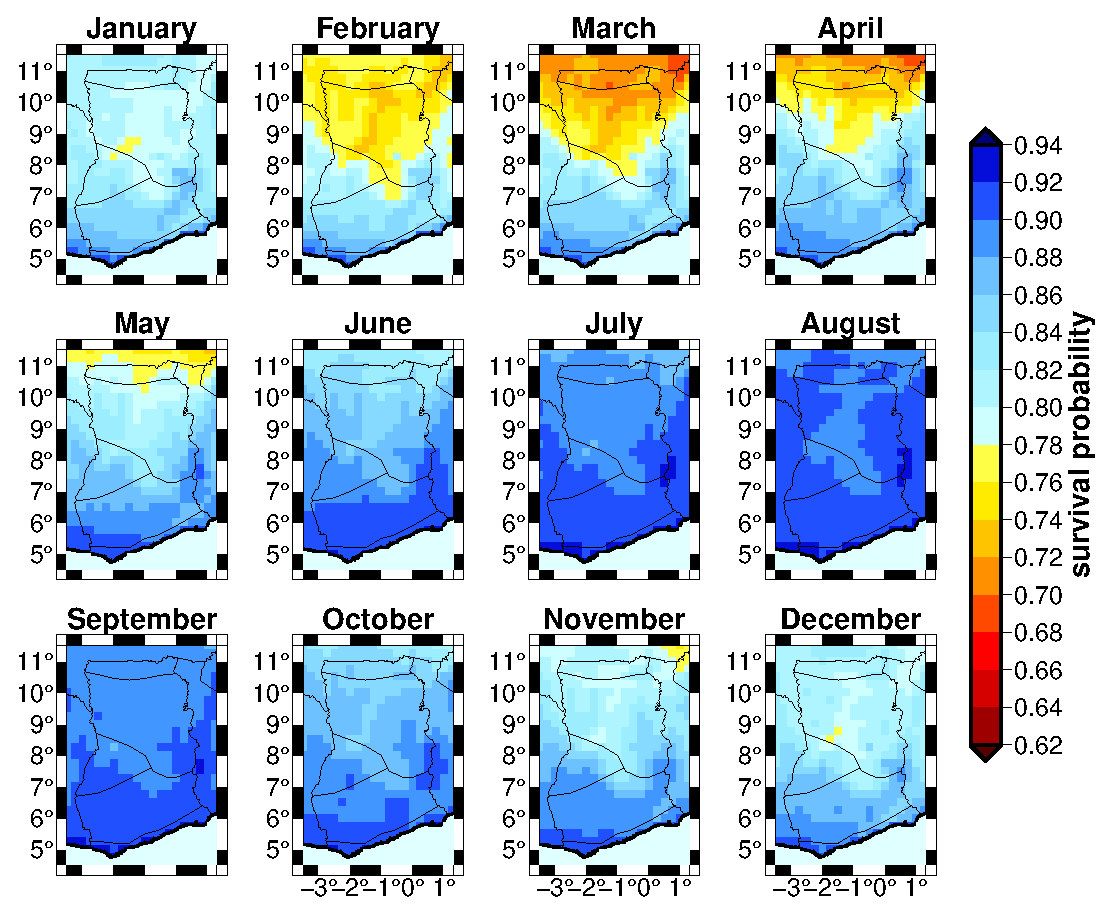
\includegraphics[width=15cm,height=15cm]{survp_era5.eps}
\caption{The spatial patterns of vector survival probabilities on monthly time scale}
\label{fig:3:1}
\end{center}
\end{figure}

In figure \ref{fig:3:2}, we present our findings regarding the duration required for parasite development within mosquitoes across different months of the year. We observe that in the Northern regions of the country, during the months of February, March, and April, the parasite development within mosquitoes takes a relatively shorter period, ranging from 5 to 6 days. In contrast, the Southern regions exhibit a longer duration, with parasite development requiring 6 to 8 days during the same months. Transitioning into the months of November, December, January, and May, we note an increase in the duration required for parasite development, although this increase is not as significant when compared to the remaining months (June, July, August, September, and October). In the Northern regions, the transition period extends from 6 to 7 days, while in the Southern regions, it ranges from 7 to 9 days. The months of June and October display intermediate values, with parasite development taking 7 to 8 days in the Northern regions and 8 to 10 days in the Southern regions. July, August, and September present the longest duration for parasite development, ranging from 8 to 12 days. Among these three months, July and September observe the shortest development period in the Northern part of the country in July and in the transition belt in September, with both registering 8 days. In contrast, August stands out as the month with the lengthiest development period throughout the entire country, spanning from 10 to 12 days, with peaks observed in the extreme south and the central regions along the Ghana-Togo border.

%Extrinsic Incubation Period
\begin{figure}[ht]
\begin{center}
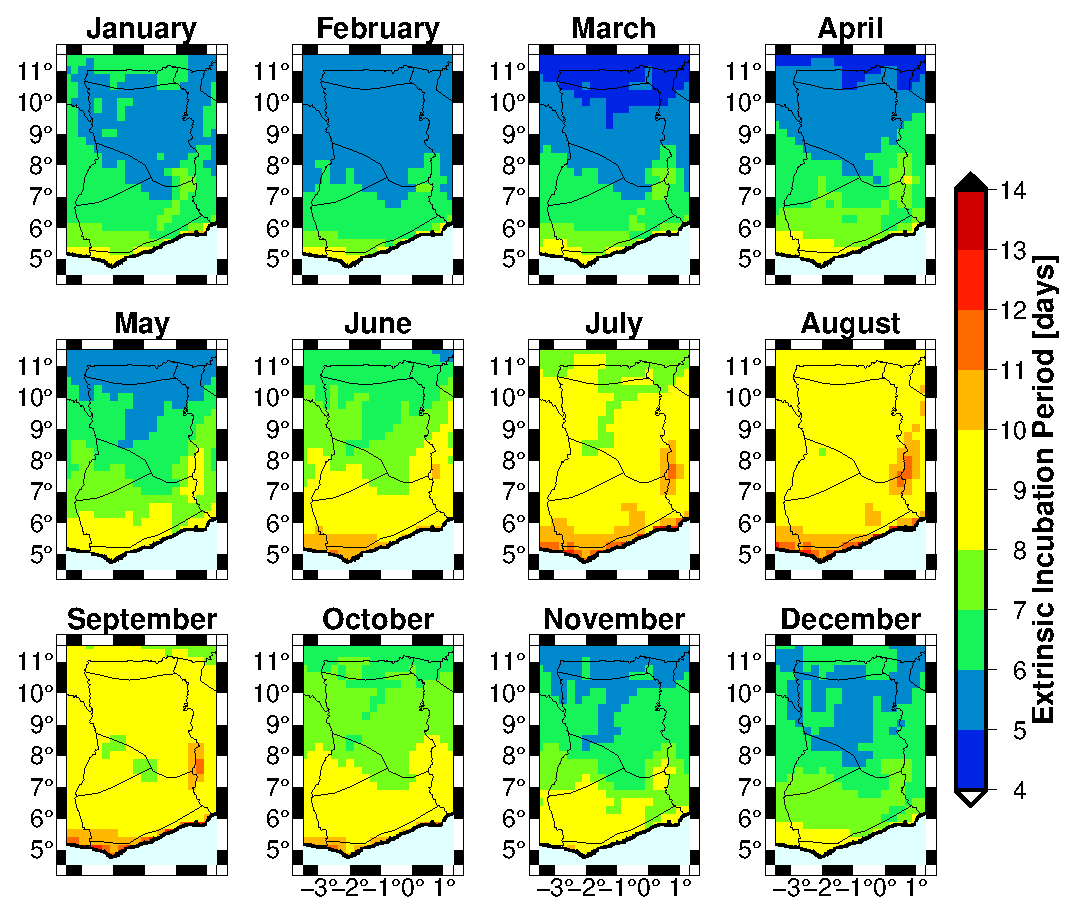
\includegraphics[width=15cm,height=15cm]{eip_era5.eps}
\caption{The spatial patterns of EIP on monthly time scale}
\label{fig:3:2}
\end{center}
\end{figure}

%Vectorial capacity
%\begin{figure}[ht]
%\begin{center}
%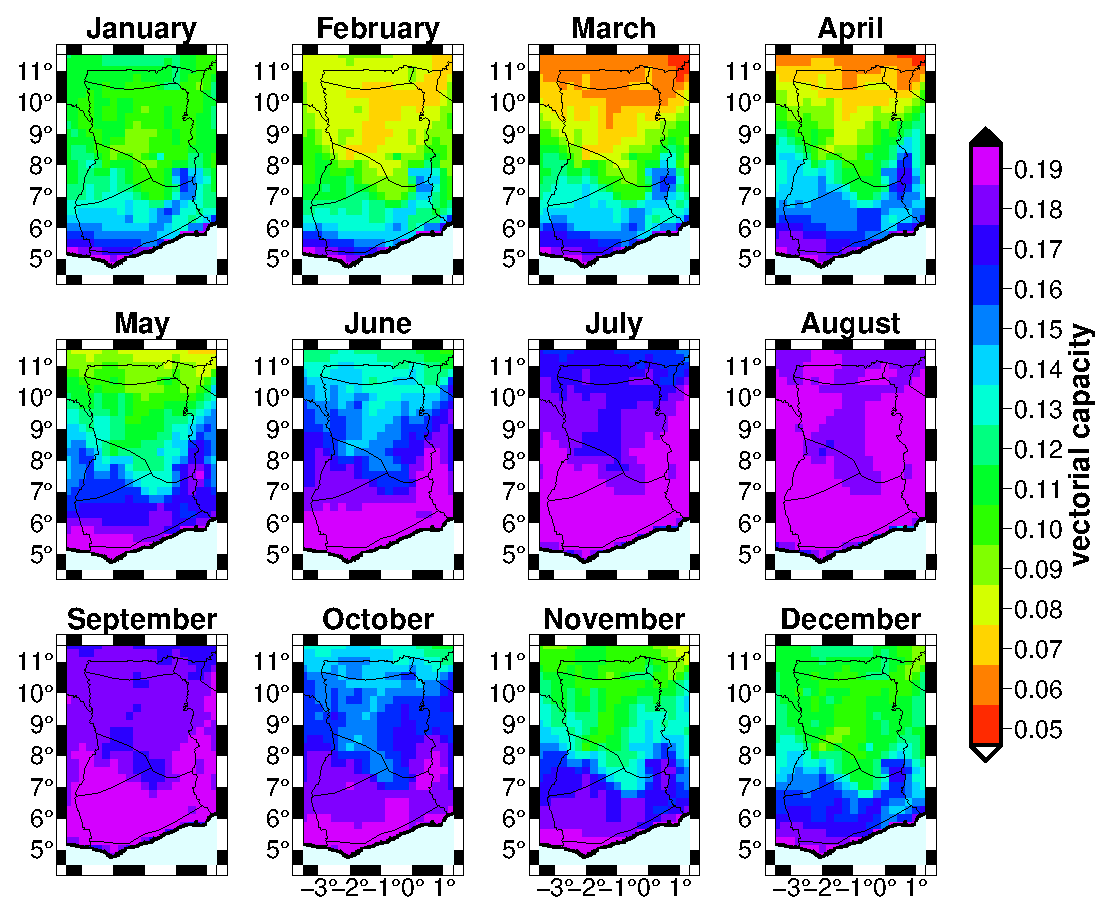
\includegraphics[width=15cm,height=15cm]{vc_era5.eps}
%\caption{The spatial patterns of vectorial capacity on monthly time scale}
%\label{fig:3:3}
%\end{center}
%\end{figure}
Considering three distinct climate periods, we sought to estimate the average duration of malaria transmission in a typical year. Figure\ref{fig:3:4} provides a visual representation of the total number of months during which malaria transmission occurs in the current climate period (1991-2020), as well as projections for the near and far future. During the current climate period, malaria transmission is predominantly concentrated in the southern regions of the country, where it occurs year-round. Notably, the Coastal regions stand out as areas with continuous transmission throughout the entire year. Following closely are the forest zones, where malaria transmission is observed for 11 to 12 months annually. The transition regions exhibit a similar pattern, with a total of 10 to 12 months of malaria transmission within a year. Subsequently, the northern region of the country experiences a relatively lower duration of malaria transmission. Specifically, in the Savannah zone, there are 8 to 9 months of malaria transmission in a typical year, while in the Sudan Savannah, the transmission period spans from 6 to 8 months. 
Looking ahead to the near future (2031-2060), our projections indicate potential changes in the spatial distribution and the duration of malaria transmission across different regions of Ghana. In the southern region, there is an expected decrease in the number of months of malaria transmission. Specifically, the Coastal zones are projected to experience transmission for 11 months, while the Forest zones may see transmission for 10 to 11 months. The transition zones are also expected to exhibit a reduction in transmission, with periods ranging from 8 to 10 months. Conversely, the northern regions are anticipated to witness an increase in the duration of malaria transmission. In the Savannah zones, the transmission period is expected to extend from 8 to 9 months to 8 to 11 months. Similarly, in the Sudan Savannah, the transmission period is projected to increase from 6 to 8 months to 7 to 9 months. 
Looking further into the far future (2061-2090), the duration of malaria transmission remains relatively stable in the southern regions, ranging from 8 to 11 months. However, there is a notable shift in the spatial distribution within the region. Specifically, significant portions of the Forest zones are expected to experience an increase in transmission duration, now totaling 9 months. This change suggests a potential expansion of malaria transmission into areas that previously had a shorter transmission season within the southern region. The northern regions, particularly the Sudan Savannah, are projected to see a further increase in the duration of malaria transmission. The transmission period is expected to extend from 6 to 8 months to 8 to 9 months in this region. 

%transmission month
\begin{figure}[ht]
\begin{center}
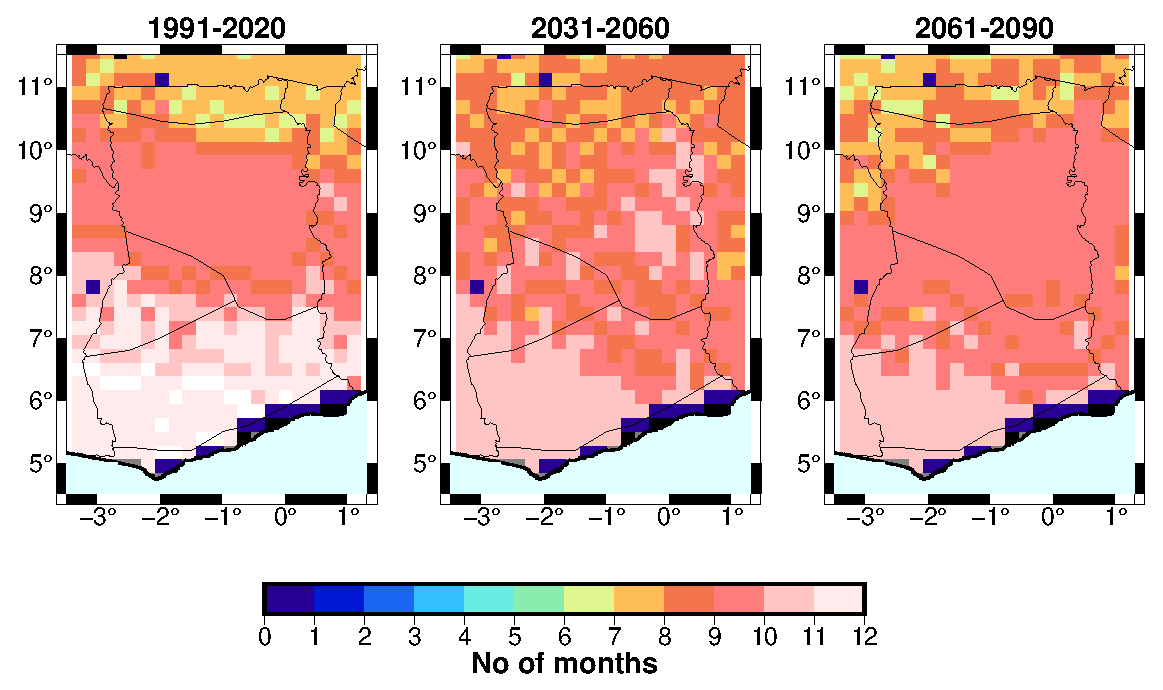
\includegraphics[width=15cm,height=9cm]{trans_months_MPI-M-MPI-ESM-LR_biascorrected.eps}
\caption{Malaria transmission months}
\label{fig:3:4}
\end{center}
\end{figure}

In Figures  \ref{fig:3:5} and \ref{fig:3:6}, we present our assessment of the averaged monthly spatial distributions of mosquito densities across the country, spanning the period from 1991-2020 and projecting into 2031-2060. Figure \ref{fig:3:5} highlights the most populated months across the entire country during the reference period (1991-2020). June, July, and October stand out as the months with the highest mosquito densities, with populations ranging from 2000 to 3500 mosquitoes per 24.42 $km^{2}$. August and September, on the other hand, record the highest number of vectors in the northern regions of the country, surpassing 3500 mosquitoes per 24.42 $km^{2}$. August witnesses this high density in the Sudan Savannah, while September experiences it in the Akuampem Mampong ranges within the transition zones. Conversely, during the months of December, January, February, and March, the country as a whole records the lowest number of mosquito vectors, with densities falling below 500 mosquitoes per 24.42 $km^{2}$. The remaining months, April, May, and November, exhibit similar characteristics, with relatively higher mosquito populations in the southern regions, although these populations are still lower compared to the peak months of June, July, and October. Projecting into the future (2031-2060), mosquito densities are expected to increase substantially to alarming levels during the months of August, September, and October, primarily in the Northern regions. These months will witness a surge in mosquito populations, which is a cause for concern. The mosquito densities during this period are projected to surpass historical records, posing potential challenges for malaria control efforts in these regions. Conversely, the months known for lower mosquito densities (December, January, February, and March) are anticipated to maintain their levels, with no significant deviations from historical patterns. However, there is some positive news in the projections as well. Densities in the months of April, May, and November are expected to experience slight reductions, particularly in the southern regions. While these months typically exhibit higher mosquito populations in the south, the projected decreases suggest a potential improvement in the mosquito situation during these periods.
\begin{figure}[ht]
\begin{center}
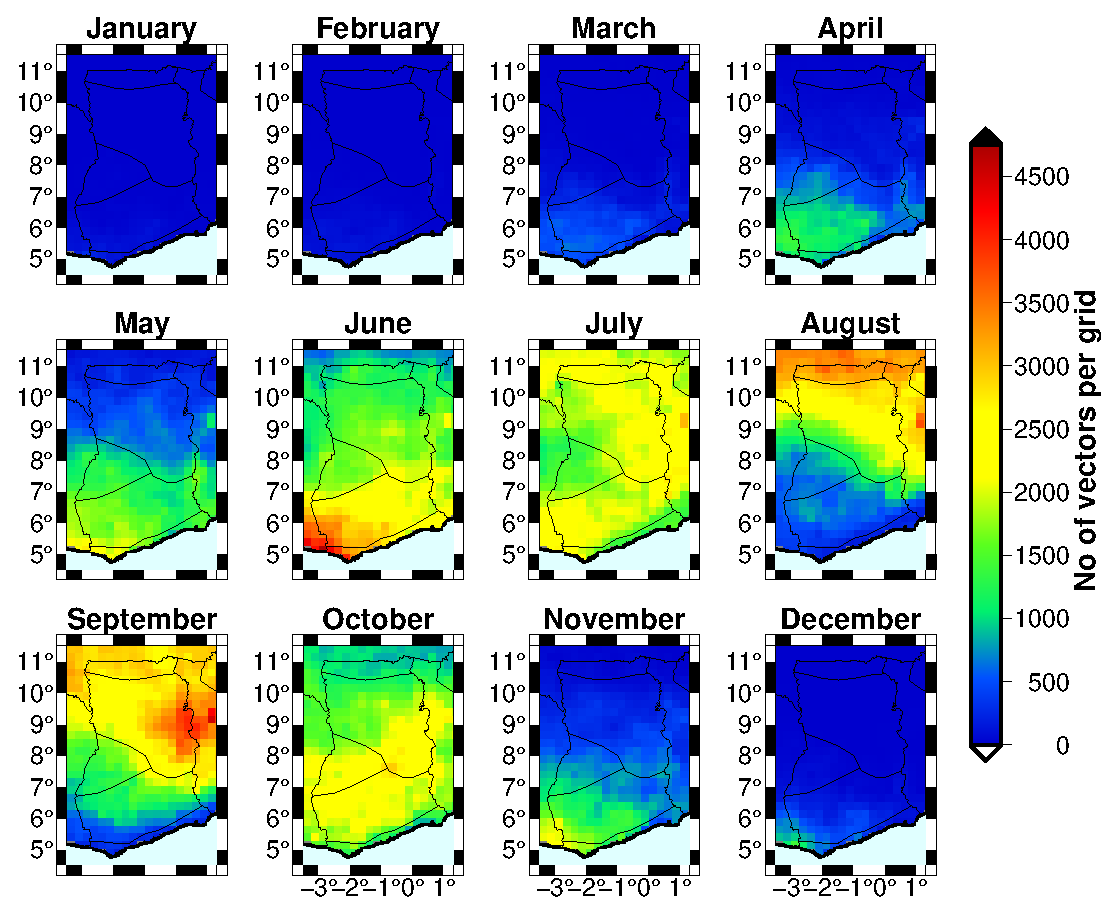
\includegraphics[width=15cm,height=15cm]{vector_chirps_ERA5.eps}
\caption{Vector distribution density from 1991-2020}
\label{fig:3:5}
\end{center}
\end{figure}
\begin{figure}[ht]
\begin{center}
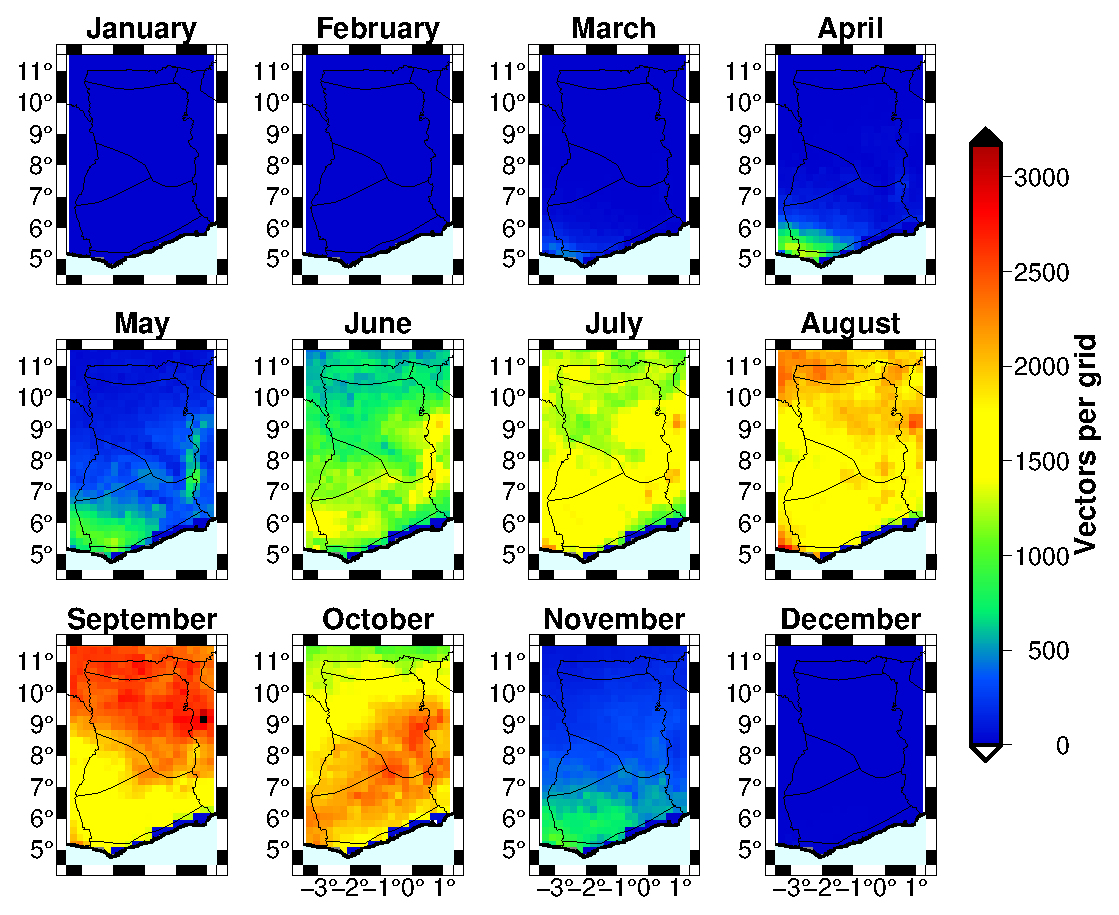
\includegraphics[width=15cm,height=15cm]{vector_MPI-M-MPI-ESM-LR_rcp26_2031-2060_biascorrected.eps}
\caption{Vector distribution density 2031-2060}
\label{fig:3:6}
\end{center}
\end{figure}

In figure \ref{fig:3:7}, we present an analysis of the average number of infectious bites received in a month from 1991-2020. Within the twelve months, the highest number of infectious bites was observed in October, around the south-eastern parts of the guinea Savannah, followed by September in the Sudan and north eastern regions of the guinea Savannah. August, July and June follows in a chronological order, with 70,60 and 50 maximum of infectious bite rate respectively. Throughout the country the months of December, January, February, March and April receives relatively low values of EIR in a typical year. Among the twelve months examined, October emerges as the month with the highest number of infectious bites. This peak in infectious bite rates is primarily concentrated in the southeastern parts of the Guinea Savannah region. Following closely, September records the second-highest number of infectious bites, particularly in the Sudan and northeastern regions of the Guinea Savannah. August, July, and June sequentially follow with decreasing maximum infectious bite rates of 70, 60, and 50, respectively. These months collectively represent a period of heightened malaria transmission risk in various regions of the country. In contrast, the months of December, January, February, March, and April receive relatively low values of Entomological Inoculation Rate (EIR) in a typical year. During these months, the risk of infectious mosquito bites is comparatively lower nationwide.
\begin{figure}[ht]
\begin{center}
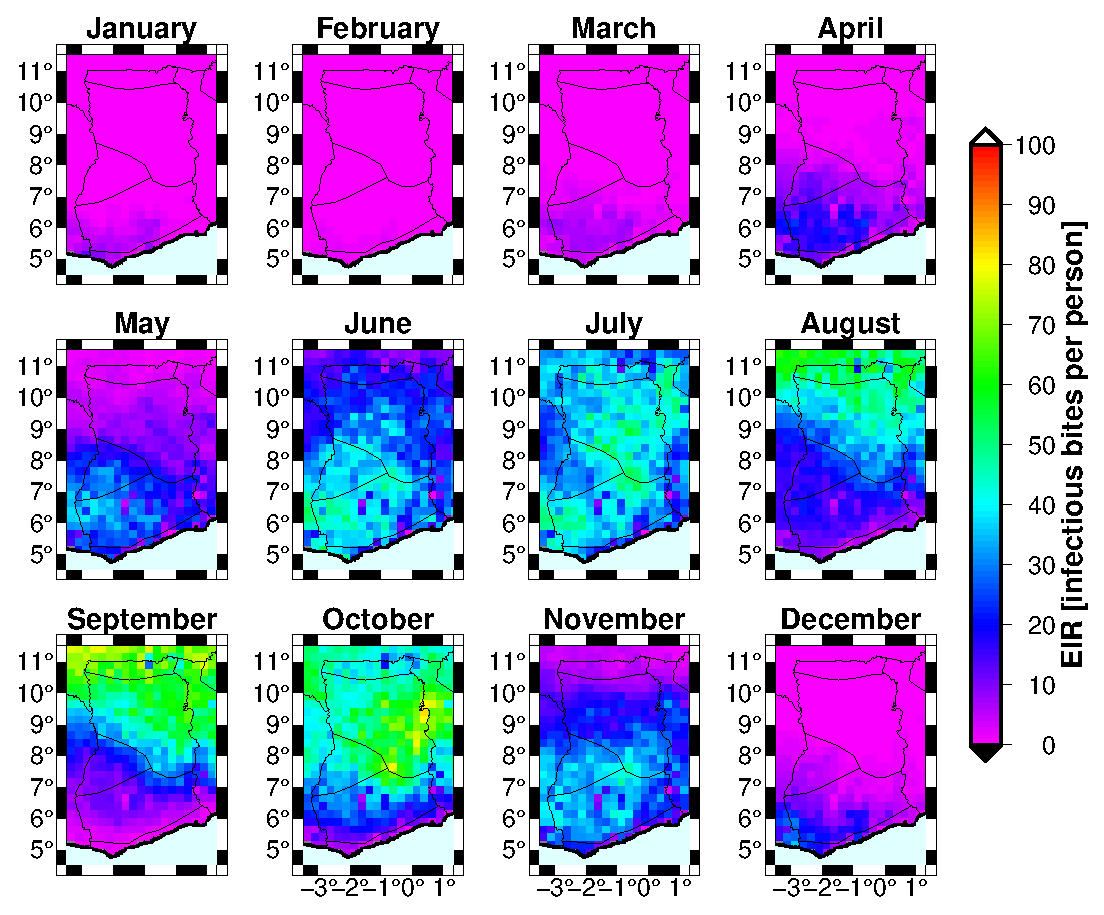
\includegraphics[width=15cm,height=15cm]{EIR_chirps_ERA5.eps}
\caption{Spatio-temporal distribution of EIR from 1991-2020}
\label{fig:3:7}
\end{center}
\end{figure}
Looking ahead into the future (2031-2060) as can be seen in figure \ref{fig:3:8}, our projections indicate significant changes in the spatial and temporal distribution of the number of infectious mosquito bites received in a square kilometer. We anticipate notable shifts in the dynamics of infectious bites. September and October are expected to experience a substantial increase in infectious bites, particularly in the northern regions of the country. On the positive side, the remaining months are expected to maintain a relatively stable EIR nationwide. This stability suggests that the risk of infectious mosquito bites during these months will not undergo significant changes compared to historical patterns.
\begin{figure}[ht]
\begin{center}
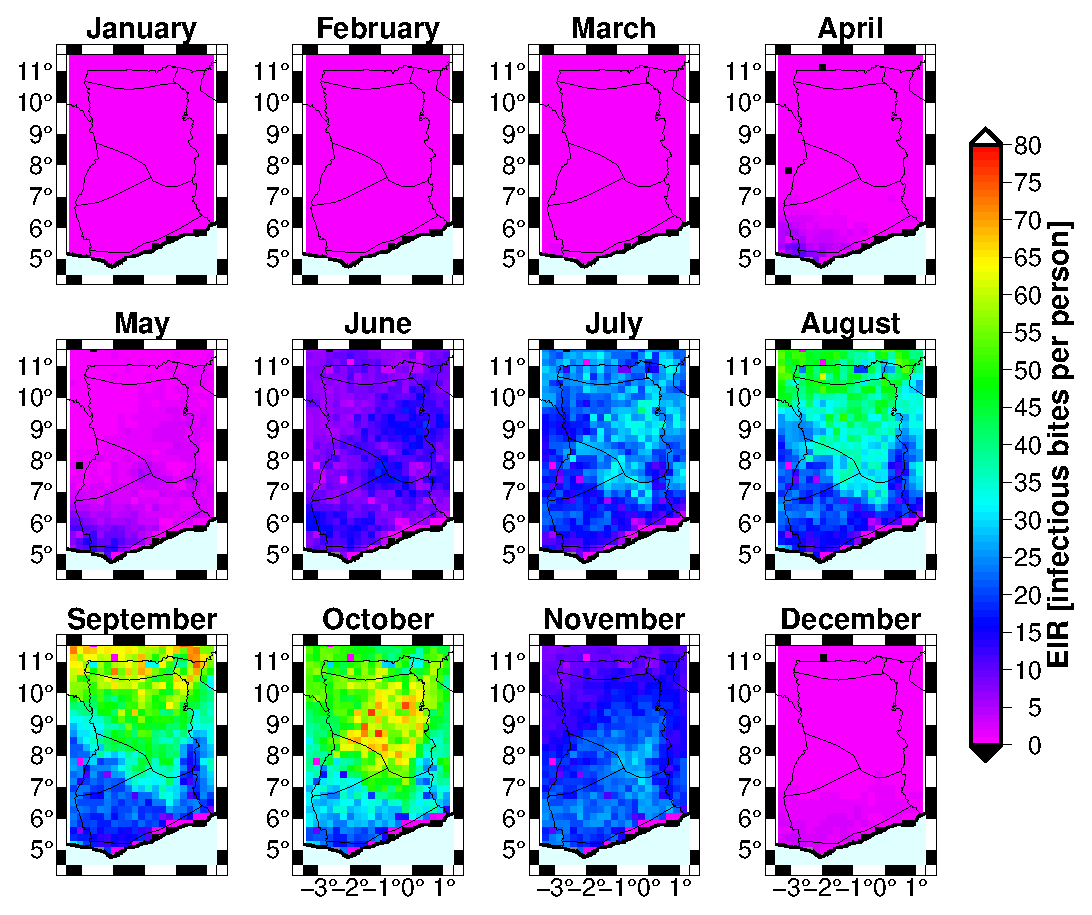
\includegraphics[width=15cm,height=15cm]{EIR_MPI-M-MPI-ESM-LR_rcp26_2031-2060_biascorrected.eps}
\caption{Spatio-temporal distribution of EIR from 2031-2060}
\label{fig:3:8}
\end{center}
\end{figure}

\section{Discussion}
In this study, we developed a climate based malaria modelling framework to enhance malaria vector surveillance and inform decision-making strategies in Ghana by uncovering a naunced picture of the spatial and temporal variations in the key factors influencing malaria risk. Our analysis unequivocally demonstrates that malaria vectors exhibit a higher susceptibility to thrive in the southern regions of Ghana, a finding that aligns seamlessly with the assessment conducted by \citep{hinne2021larval} on the distribution of malaria vectors across distinct ecological zones within Ghana. Delving deeper into the geographical disparities, we observe a remarkable decline in the risk of vectors thriving during typical dry months in the northern region. The rationale behind this decline lies in the apparent scarcity of suitable breeding grounds for mosquitoes in these sectors, leading to a notable reduction in their populations. This starkly contrasts with the situation in the southern region, where even during the dry season, the occasional rainfall bestows a significantly higher probability for mosquito survival. Temperature and humidity play crucial roles in this phenomenon as well. As one moves northward in Ghana, temperatures tend to rise, with occasional spikes of up to 40$^{o}C$. Mosquitoes, known for their ability to withstand colder temperatures (less than 40$^o$C), find the more favorable conditions in the south, resulting in a diminished mosquito population during the specified months, as depicted in Figure 5. Further narrowing our focus to the months spanning from November to March, we unveil a consistent trend of low mosquito presence throughout the country. The prevailing weather conditions during this period are not conducive to the proliferation of malaria, leading to a reduced mosquito population and subsequently fewer instances of biting and infectious bites. The empirical evidence supporting this trend is underscored in Figure 7.





These findings enable the identification of high-risk areas and critical timeframes for malaria transmission.





These projections highlight the dynamic nature of malaria transmission and the need for adaptive strategies to address changing patterns. It is essential to closely monitor these developments and adjust malaria control efforts accordingly, with a focus on both maintaining progress in areas with decreasing transmission and implementing targeted interventions to mitigate the spread of malaria in regions experiencing extended transmission seasons.





 Additionally, the data we have produced can guide the design of vector control strategies tailored to specific regions and seasons. The projections for the future also serve as an early warning system, alerting health authorities to potential shifts in transmission dynamics. This allows for proactive planning and rapid response, helping to prevent outbreaks and reduce the overall malaria burden.





\section{Conclusion}
This research aims to contribute to the understanding of the intricate relationship between climate and malaria transmission in Ghana. The outcomes of this study will include:

    Climate-based Model: A robust predictive model that accurately forecasts the distribution and abundance of malaria vectors based on climate conditions.

    Insights into Climate-Vector-Disease Nexus: A better understanding of how climate influences vector population dynamics and disease transmission, allowing for more targeted interventions.

    Climate Change Impact Assessment: Insights into the potential impact of climate change on malaria transmission, enabling proactive adaptation strategies.

    Policy Recommendations: Actionable recommendations for public health authorities to optimize vector surveillance and control efforts based on climate-driven predictions.







\section{Additional Requirements}

For additional requirements for specific article types and further information please refer to \href{http://www.frontiersin.org/about/AuthorGuidelines#AdditionalRequirements}{Author Guidelines}.

\section*{Conflict of Interest Statement}
%All financial, commercial or other relationships that might be perceived by the academic community as representing a potential conflict of interest must be disclosed. If no such relationship exists, authors will be asked to confirm the following statement: 

The authors declare that the research was conducted in the absence of any commercial or financial relationships that could be construed as a potential conflict of interest.

\section*{Author Contributions}

The Author Contributions section is mandatory for all articles, including articles by sole authors. If an appropriate statement is not provided on submission, a standard one will be inserted during the production process. The Author Contributions statement must describe the contributions of individual authors referred to by their initials and, in doing so, all authors agree to be accountable for the content of the work. Please see  \href{https://www.frontiersin.org/about/policies-and-publication-ethics#AuthorshipAuthorResponsibilities}{here} for full authorship criteria.

\section*{Funding}
Details of all funding sources should be provided, including grant numbers if applicable. Please ensure to add all necessary funding information, as after publication this is no longer possible.

\section*{Acknowledgments}
This is a short text to acknowledge the contributions of specific colleagues, institutions, or agencies that aided the efforts of the authors.

\section*{Supplemental Data}
 \href{http://home.frontiersin.org/about/author-guidelines#SupplementaryMaterial}{Supplementary Material} should be uploaded separately on submission, if there are Supplementary Figures, please include the caption in the same file as the figure. LaTeX Supplementary Material templates can be found in the Frontiers LaTeX folder.

\section*{Data Availability Statement}
\noindent The Climate Hazards Infra-Red Precipitation (CHIRPs) database can be found in the Climate Hazard Center repository at \url{https://www.chc.ucsb.edu/data/chirps}. \\
The 2m temperature data from the European Centre for Medium-Range Weather Forecasts (ECMWF) Re-Analysis, 5th generation (ERA5) is available at the copernicus data resporsitory under the link: \url{https://cds.climate.copernicus.eu/cdsapp#!/dataset/reanalysis-era5-single-levels?tab=form}. \\

The Coordinated Regional Climate Downscaling Experiment (CORDEX) simulation framework database is available at the CORDEX data reporsitory at \url{https://cordex.org/data-access/cordex-data-on-esgf/}

%The datasets [GENERATED/ANALYZED] for this study can be found in the [NAME OF REPOSITORY] [LINK].
% Please see the availability of data guidelines for more information, at https://www.frontiersin.org/about/author-guidelines#AvailabilityofData

\bibliographystyle{Frontiers-Harvard} %  Many Frontiers journals use the Harvard referencing system (Author-date), to find the style and resources for the journal you are submitting to: https://zendesk.frontiersin.org/hc/en-us/articles/360017860337-Frontiers-Reference-Styles-by-Journal. For Humanities and Social Sciences articles please include page numbers in the in-text citations 
%\bibliographystyle{Frontiers-Vancouver} % Many Frontiers journals use the numbered referencing system, to find the style and resources for the journal you are submitting to: https://zendesk.frontiersin.org/hc/en-us/articles/360017860337-Frontiers-Reference-Styles-by-Journal
\bibliography{References}

%%% Make sure to upload the bib file along with the tex file and PDF
%%% Please see the test.bib file for some examples of references

\section*{Figure captions}

%%% Please be aware that for original research articles we only permit a combined number of 15 figures and tables, one figure with multiple subfigures will count as only one figure.
%%% Use this if adding the figures directly in the mansucript, if so, please remember to also upload the files when submitting your article
%%% There is no need for adding the file termination, as long as you indicate where the file is saved. In the examples below the files (logo1.eps and logos.eps) are in the Frontiers LaTeX folder
%%% If using *.tif files convert them to .jpg or .png
%%%  NB logo1.eps is required in the path in order to correctly compile front page header %%%

\begin{figure}[h!]
\begin{center}

\includegraphics[width=10cm]{logo1}% This is a *.eps file
\end{center}
\caption{ Enter the caption for your figure here.  Repeat as  necessary for each of your figures}\label{fig:1}
\end{figure}

\setcounter{figure}{2}
\setcounter{subfigure}{0}
\begin{subfigure}
\setcounter{figure}{2}
\setcounter{subfigure}{0}
    \centering
    \begin{minipage}[b]{0.5\textwidth}
        
\includegraphics[width=\linewidth]{logo1.eps}
        \caption{This is Subfigure 1.}
        \label{fig:Subfigure 1}
    \end{minipage}  
   
\setcounter{figure}{2}
\setcounter{subfigure}{1}
    \begin{minipage}[b]{0.5\textwidth}
        
\includegraphics[width=\linewidth]{logo2.eps}
        \caption{This is Subfigure 2.}
        \label{fig:Subfigure 2}
    \end{minipage}

\setcounter{figure}{2}
\setcounter{subfigure}{-1}
    \caption{Enter the caption for your subfigure here. \textbf{(A)} This is the caption for Subfigure 1. \textbf{(B)} This is the caption for Subfigure 2.}
    \label{fig: subfigures}
\end{subfigure}

%%% If you don't add the figures in the LaTeX files, please upload them when submitting the article.
%%% Frontiers will add the figures at the end of the provisional pdf automatically
%%% The use of LaTeX coding to draw Diagrams/Figures/Structures should be avoided. They should be external callouts including graphics.

\end{document}
